\documentclass{article}

\PassOptionsToPackage{numbers,compress,sort}{natbib}
\usepackage[preprint]{neurips_2026}

\usepackage[utf8]{inputenc}
\usepackage[T1]{fontenc}
\usepackage[hidelinks]{hyperref}
\usepackage{url}
\usepackage{booktabs}
\usepackage{amsfonts}
\usepackage{amssymb}
\usepackage{amsmath}
\usepackage{microtype}
\usepackage{graphicx}
\usepackage{subcaption}
\usepackage{tikz}
\usetikzlibrary{positioning,arrows.meta}

\newcommand{\ExploitAcceptedBad}{0}
\newcommand{\ExploitBestNonRef}{0.394}
\newcommand{\ExploitBlindAccess}{0.378}
\newcommand{\ExploitBoomAccess}{0.394}
\newcommand{\ExploitFirstNegative}{7}
\newcommand{\ExploitMaintTwoGap}{+0.0009}
\newcommand{\ExploitMaintZeroGap}{$-$0.0084}
\newcommand{\ExploitMaintZeroN}{16}
\newcommand{\ExploitMaintZeroP}{0.011}
\newcommand{\ExploitMaintZeroWins}{13}
\newcommand{\ExploitNothingDebt}{$-$521.9}
\newcommand{\ExploitNothingFirstNegative}{10}
\newcommand{\ExploitPlanDoneYear}{7}
\newcommand{\ExploitRefCI}{0.947--0.983}
\newcommand{\ExploitRefDebt}{$-$918.6}
\newcommand{\ExploitRefMean}{0.966}
\newcommand{\ExploitRefOverOne}{3}
\newcommand{\ExploitStopFive}{0.757}
\newcommand{\ExploitStopSevenGap}{0}
\newcommand{\ExploitStopThree}{0.149}
\newcommand{\agentBoomEarly}{2}
\newcommand{\agentBoomHits}{4}
\newcommand{\agentForecastMax}{38}
\newcommand{\agentForecastMin}{28}
\newcommand{\agentGetStateMax}{8}
\newcommand{\agentGetStateMin}{7}
\newcommand{\agentLostC}{73.5}
\newcommand{\agentMinMax}{7}
\newcommand{\agentMinMin}{6}
\newcommand{\agentN}{5}
\newcommand{\agentScoreMean}{0.77}
\newcommand{\agentSeeds}{0 to 4}
\newcommand{\agentUsdMax}{0.43}
\newcommand{\agentUsdMin}{0.33}
\newcommand{\bestPctMax}{60.9}
\newcommand{\bestPctMin}{16.9}
\newcommand{\cfAccessAccepted}{1/5}
\newcommand{\cfAccessDiff}{0.004}
\newcommand{\cfAccessGapShare}{0.018}
\newcommand{\cfBothDiff}{$-$0.297}
\newcommand{\cfBothGapShare}{$-$1.45}
\newcommand{\cfMaintOneDiff}{$-$0.185}
\newcommand{\cfMaintOneGapShare}{$-$0.90}
\newcommand{\cfRefMaintTwoDiff}{$-$0.280}
\newcommand{\cfRefMaintTwoGapShare}{1.36}
\newcommand{\evoBcAcc}{0.67}
\newcommand{\evoBcAccAt}{0}
\newcommand{\evoBcAccScore}{0.91}
\newcommand{\evoBcAccShare}{0.67}
\newcommand{\evoBcAccYear}{2029}
\newcommand{\evoBcBoom}{0.49}
\newcommand{\evoBcBoomZero}{0.44}
\newcommand{\evoBcBuildsOne}{2.0}
\newcommand{\evoBcDistinct}{11}
\newcommand{\evoBcDistinctZero}{10}
\newcommand{\evoBcEnt}{0.04}
\newcommand{\evoBcEntZero}{0.12}
\newcommand{\evoBcEps}{960}
\newcommand{\evoBcEpsOne}{80}
\newcommand{\evoBcMaxAcc}{1.00}
\newcommand{\evoBcMone}{1.00}
\newcommand{\evoBcMtwoOne}{0.00}
\newcommand{\evoBcNoAccUntil}{0}
\newcommand{\evoBcOta}{0.44}
\newcommand{\evoBcOtaZero}{0.50}
\newcommand{\evoBcScore}{0.95}
\newcommand{\evoBcScoreOne}{0.88}
\newcommand{\evoBcScoreZero}{0.91}
\newcommand{\evoColdAcc}{0.20}
\newcommand{\evoColdAccAt}{1120}
\newcommand{\evoColdAccScore}{0.70}
\newcommand{\evoColdAccShare}{0.14}
\newcommand{\evoColdAccYear}{2034}
\newcommand{\evoColdBoom}{0.27}
\newcommand{\evoColdBoomZero}{0.00}
\newcommand{\evoColdBuildsOne}{7.8}
\newcommand{\evoColdDistinct}{5}
\newcommand{\evoColdDistinctZero}{1}
\newcommand{\evoColdEnt}{0.81}
\newcommand{\evoColdEntZero}{4.63}
\newcommand{\evoColdEps}{5280}
\newcommand{\evoColdEpsOne}{80}
\newcommand{\evoColdMaxAcc}{0.20}
\newcommand{\evoColdMone}{0.00}
\newcommand{\evoColdMtwoOne}{1.00}
\newcommand{\evoColdNoAccUntil}{1040}
\newcommand{\evoColdOta}{0.19}
\newcommand{\evoColdOtaZero}{0.00}
\newcommand{\evoColdScore}{0.71}
\newcommand{\evoColdScoreOne}{0.23}
\newcommand{\evoColdScoreZero}{-0.02}
\newcommand{\evoGumbelAcc}{0.00}
\newcommand{\evoGumbelBoom}{0.00}
\newcommand{\evoGumbelBoomZero}{0.00}
\newcommand{\evoGumbelBuildsOne}{4.6}
\newcommand{\evoGumbelDistinct}{14}
\newcommand{\evoGumbelDistinctZero}{1}
\newcommand{\evoGumbelEnt}{2.78}
\newcommand{\evoGumbelEntZero}{4.63}
\newcommand{\evoGumbelEps}{72}
\newcommand{\evoGumbelEpsOne}{6}
\newcommand{\evoGumbelMaxAcc}{0.00}
\newcommand{\evoGumbelMone}{0.15}
\newcommand{\evoGumbelMtwoOne}{0.78}
\newcommand{\evoGumbelOta}{0.00}
\newcommand{\evoGumbelOtaZero}{0.00}
\newcommand{\evoGumbelScore}{0.13}
\newcommand{\evoGumbelScoreOne}{0.21}
\newcommand{\evoGumbelScoreZero}{-0.02}
\newcommand{\failBlockedAgent}{12.8}
\newcommand{\failBlockedRef}{13.0}
\newcommand{\failBoomAgent}{4}
\newcommand{\failBoomEarlyAgent}{2}
\newcommand{\failBoomEarlyRef}{2}
\newcommand{\failBoomNeverActed}{11}
\newcommand{\failBoomRef}{6}
\newcommand{\failBoomTotal}{15}
\newcommand{\failCallsForecast}{34.2}
\newcommand{\failCallsGetState}{7.4}
\newcommand{\failForecastAccess}{8.4}
\newcommand{\failForecastAccessUnbuilt}{3.6}
\newcommand{\failJaccardAgent}{0.72}
\newcommand{\failJaccardRef}{0.44}
\newcommand{\failLagYears}{4.2}
\newcommand{\failMaintTwoShare}{6.2\%}
\newcommand{\failMentionYear}{2028}
\newcommand{\failRebuildShareAgent}{77\%}
\newcommand{\failRebuildShareRef}{82\%}
\newcommand{\gapIntelHi}{0.380}
\newcommand{\gapIntelLo}{0.047}
\newcommand{\gapIntelMean}{0.205}
\newcommand{\gapIntelSignP}{0.031}
\newcommand{\gapIntelWins}{5/5}
\newcommand{\gapRlA}{43}
\newcommand{\greedyFiveMOne}{0.28}
\newcommand{\greedyFiveMTwo}{0.57}
\newcommand{\grpoBoomHitEnd}{0.22}
\newcommand{\grpoBoomHitMax}{0.34}
\newcommand{\grpoBoomShare}{0.31}
\newcommand{\grpoDropFirst}{\texttt{keha2-north}, \texttt{espoonvayla-mid}, \texttt{kivenlahti-bridge}, \texttt{keha2-turunvayla-junction}, \texttt{kauklahti-access}}
\newcommand{\grpoFinal}{0.83}
\newcommand{\grpoFlatAt}{80}
\newcommand{\grpoKept}{\texttt{espoonvayla-2x2}, \texttt{kiviruukki-access}, \texttt{otaniemi-access}}
\newcommand{\grpoKeptAt}{50}
\newcommand{\grpoLastStep}{90}
\newcommand{\grpoMtwoAt}{10}
\newcommand{\grpoOneAt}{60}
\newcommand{\grpoPlan}{\texttt{otaniemi-access}, \texttt{kiviruukki-access}, \texttt{espoonvayla-2x2}}
\newcommand{\grpoScoreEnd}{0.83}
\newcommand{\grpoScoreWarmS}{0.19}
\newcommand{\grpoSdWarm}{8.0}
\newcommand{\grpoSteps}{90}
\newcommand{\grpoValid}{1.00}
\newcommand{\grpoValidAt}{20}
\newcommand{\grpoWarm}{0.19}
\newcommand{\grpoZero}{0.00}
\newcommand{\hoGap}{3.6}
\newcommand{\hoN}{32}
\newcommand{\hoRl}{34.3}
\newcommand{\hoRlEval}{37.9}
\newcommand{\hoSeeds}{16 to 47}
\newcommand{\hoWinPlanner}{31}
\newcommand{\hoWinReactive}{32}
\newcommand{\jamFew}{10}
\newcommand{\jamFewGap}{0.17}
\newcommand{\jamFewMinWith}{0.35}
\newcommand{\jamFewMinWithout}{0.08}
\newcommand{\jamMany}{194}
\newcommand{\jamManyGap}{0.01}
\newcommand{\nBooms}{15}
\newcommand{\nothingAbsMax}{0.003}
\newcommand{\nothingRatioMax}{8.3}
\newcommand{\nothingRatioMin}{2.0}
\newcommand{\reactiveMOne}{0.55}
\newcommand{\reactiveMTwo}{0.56}
\newcommand{\refoldLostC}{76.0}
\newcommand{\refrlGap}{0.00}
\newcommand{\refrlN}{5}
\newcommand{\rlBoomAny}{12}
\newcommand{\rlBoomEarly}{9}
\newcommand{\rlLostC}{72.8}
\newcommand{\rlN}{16}
\newcommand{\rlScore}{0.97}
\newcommand{\rlcheckScore}{0.40}
\newcommand{\rlsearchScore}{0.96}
\newcommand{\rlsearchWorse}{7, 15}
\newcommand{\testDeploySaved}{34.3}
\newcommand{\testDeploySavedHi}{39.5}
\newcommand{\testDeploySavedLo}{29.2}
\newcommand{\testDeployWorst}{14.9}
\newcommand{\testGreedyFiveMTwoN}{32}
\newcommand{\testGreedyFiveMTwoSaved}{12.2}
\newcommand{\testGreedyFiveMTwoSavedHi}{14.9}
\newcommand{\testGreedyFiveMTwoSavedLo}{9.9}
\newcommand{\testGreedyFiveMTwoSignP}{7.7e-09}
\newcommand{\testGreedyFiveMTwoWilcoxonP}{4.7e-10}
\newcommand{\testGreedyFiveMTwoWins}{31}
\newcommand{\testGreedyFiveMTwoWorst}{4.8}
\newcommand{\testGreedyFiveN}{32}
\newcommand{\testGreedyFiveSaved}{7.6}
\newcommand{\testGreedyFiveSavedHi}{8.6}
\newcommand{\testGreedyFiveSavedLo}{6.6}
\newcommand{\testGreedyFiveSignP}{2.3e-10}
\newcommand{\testGreedyFiveWilcoxonP}{2.3e-10}
\newcommand{\testGreedyFiveWins}{32}
\newcommand{\testGreedyFiveWorst}{1.6}
\newcommand{\testGreedyOneMTwoN}{32}
\newcommand{\testGreedyOneMTwoSaved}{10.0}
\newcommand{\testGreedyOneMTwoSavedHi}{11.1}
\newcommand{\testGreedyOneMTwoSavedLo}{9.0}
\newcommand{\testGreedyOneMTwoSignP}{2.3e-10}
\newcommand{\testGreedyOneMTwoWilcoxonP}{2.3e-10}
\newcommand{\testGreedyOneMTwoWins}{32}
\newcommand{\testGreedyOneMTwoWorst}{5.5}
\newcommand{\testGreedyOneN}{32}
\newcommand{\testGreedyOneSaved}{9.8}
\newcommand{\testGreedyOneSavedHi}{10.9}
\newcommand{\testGreedyOneSavedLo}{8.8}
\newcommand{\testGreedyOneSignP}{2.3e-10}
\newcommand{\testGreedyOneWilcoxonP}{2.3e-10}
\newcommand{\testGreedyOneWins}{32}
\newcommand{\testGreedyOneWorst}{5.3}
\newcommand{\testNothingN}{32}
\newcommand{\testNothingSaved}{0.0}
\newcommand{\testNothingSavedHi}{0.0}
\newcommand{\testNothingSavedLo}{0.0}
\newcommand{\testNothingSignP}{2.3e-10}
\newcommand{\testNothingWilcoxonP}{2.3e-10}
\newcommand{\testNothingWins}{32}
\newcommand{\testNothingWorst}{0.0}
\newcommand{\testPlannerN}{32}
\newcommand{\testPlannerSaved}{31.1}
\newcommand{\testPlannerSavedHi}{36.2}
\newcommand{\testPlannerSavedLo}{26.2}
\newcommand{\testPlannerSignP}{7.7e-09}
\newcommand{\testPlannerWilcoxonP}{8.6e-08}
\newcommand{\testPlannerWins}{31}
\newcommand{\testPlannerWorst}{13.2}
\newcommand{\testRandomN}{32}
\newcommand{\testRandomSaved}{4.6}
\newcommand{\testRandomSavedHi}{5.4}
\newcommand{\testRandomSavedLo}{3.8}
\newcommand{\testRandomSignP}{2.3e-10}
\newcommand{\testRandomWilcoxonP}{2.3e-10}
\newcommand{\testRandomWins}{32}
\newcommand{\testRandomWorst}{-0.1}
\newcommand{\testReactiveMTwoN}{32}
\newcommand{\testReactiveMTwoSaved}{20.6}
\newcommand{\testReactiveMTwoSavedHi}{24.9}
\newcommand{\testReactiveMTwoSavedLo}{16.6}
\newcommand{\testReactiveMTwoSignP}{2.3e-10}
\newcommand{\testReactiveMTwoWilcoxonP}{2.3e-10}
\newcommand{\testReactiveMTwoWins}{32}
\newcommand{\testReactiveMTwoWorst}{7.6}
\newcommand{\testReactiveN}{32}
\newcommand{\testReactiveSaved}{19.9}
\newcommand{\testReactiveSavedHi}{24.3}
\newcommand{\testReactiveSavedLo}{16.0}
\newcommand{\testReactiveSignP}{2.3e-10}
\newcommand{\testReactiveWilcoxonP}{2.3e-10}
\newcommand{\testReactiveWins}{32}
\newcommand{\testReactiveWorst}{6.9}
\newcommand{\validationDeploySaved}{37.9}
\newcommand{\validationDeploySavedHi}{44.5}
\newcommand{\validationDeploySavedLo}{31.1}
\newcommand{\validationDeployWorst}{16.5}
\newcommand{\validationGreedyFiveMTwoN}{16}
\newcommand{\validationGreedyFiveMTwoSaved}{16.7}
\newcommand{\validationGreedyFiveMTwoSavedHi}{21.3}
\newcommand{\validationGreedyFiveMTwoSavedLo}{12.5}
\newcommand{\validationGreedyFiveMTwoSignP}{1.5e-05}
\newcommand{\validationGreedyFiveMTwoWilcoxonP}{1.5e-05}
\newcommand{\validationGreedyFiveMTwoWins}{16}
\newcommand{\validationGreedyFiveMTwoWorst}{5.7}
\newcommand{\validationGreedyFiveN}{16}
\newcommand{\validationGreedyFiveSaved}{8.3}
\newcommand{\validationGreedyFiveSavedHi}{9.9}
\newcommand{\validationGreedyFiveSavedLo}{6.7}
\newcommand{\validationGreedyFiveSignP}{1.5e-05}
\newcommand{\validationGreedyFiveWilcoxonP}{1.5e-05}
\newcommand{\validationGreedyFiveWins}{16}
\newcommand{\validationGreedyFiveWorst}{1.7}
\newcommand{\validationGreedyOneMTwoN}{16}
\newcommand{\validationGreedyOneMTwoSaved}{10.9}
\newcommand{\validationGreedyOneMTwoSavedHi}{12.6}
\newcommand{\validationGreedyOneMTwoSavedLo}{9.3}
\newcommand{\validationGreedyOneMTwoSignP}{1.5e-05}
\newcommand{\validationGreedyOneMTwoWilcoxonP}{1.5e-05}
\newcommand{\validationGreedyOneMTwoWins}{16}
\newcommand{\validationGreedyOneMTwoWorst}{6.0}
\newcommand{\validationGreedyOneN}{16}
\newcommand{\validationGreedyOneSaved}{10.8}
\newcommand{\validationGreedyOneSavedHi}{12.5}
\newcommand{\validationGreedyOneSavedLo}{9.2}
\newcommand{\validationGreedyOneSignP}{1.5e-05}
\newcommand{\validationGreedyOneWilcoxonP}{1.5e-05}
\newcommand{\validationGreedyOneWins}{16}
\newcommand{\validationGreedyOneWorst}{5.8}
\newcommand{\validationNothingN}{16}
\newcommand{\validationNothingSaved}{0.0}
\newcommand{\validationNothingSavedHi}{0.0}
\newcommand{\validationNothingSavedLo}{0.0}
\newcommand{\validationNothingSignP}{1.5e-05}
\newcommand{\validationNothingWilcoxonP}{1.5e-05}
\newcommand{\validationNothingWins}{16}
\newcommand{\validationNothingWorst}{0.0}
\newcommand{\validationPlannerN}{16}
\newcommand{\validationPlannerSaved}{32.8}
\newcommand{\validationPlannerSavedHi}{39.6}
\newcommand{\validationPlannerSavedLo}{26.3}
\newcommand{\validationPlannerSignP}{1.5e-05}
\newcommand{\validationPlannerWilcoxonP}{1.5e-05}
\newcommand{\validationPlannerWins}{16}
\newcommand{\validationPlannerWorst}{14.8}
\newcommand{\validationRandomN}{16}
\newcommand{\validationRandomSaved}{4.5}
\newcommand{\validationRandomSavedHi}{6.2}
\newcommand{\validationRandomSavedLo}{2.9}
\newcommand{\validationRandomSignP}{1.5e-05}
\newcommand{\validationRandomWilcoxonP}{1.5e-05}
\newcommand{\validationRandomWins}{16}
\newcommand{\validationRandomWorst}{0.0}
\newcommand{\validationReactiveMTwoN}{16}
\newcommand{\validationReactiveMTwoSaved}{21.1}
\newcommand{\validationReactiveMTwoSavedHi}{28.9}
\newcommand{\validationReactiveMTwoSavedLo}{14.6}
\newcommand{\validationReactiveMTwoSignP}{1.5e-05}
\newcommand{\validationReactiveMTwoWilcoxonP}{1.5e-05}
\newcommand{\validationReactiveMTwoWins}{16}
\newcommand{\validationReactiveMTwoWorst}{8.3}
\newcommand{\validationReactiveN}{16}
\newcommand{\validationReactiveSaved}{20.8}
\newcommand{\validationReactiveSavedHi}{28.7}
\newcommand{\validationReactiveSavedLo}{14.3}
\newcommand{\validationReactiveSignP}{1.5e-05}
\newcommand{\validationReactiveWilcoxonP}{1.5e-05}
\newcommand{\validationReactiveWins}{16}
\newcommand{\validationReactiveWorst}{8.3}

\newcommand{\shot}[1]{\includegraphics[width=\linewidth]{figs/shot_#1.jpg}}
\newcommand{\repo}{\texttt{espoo-2040}}

\title{From Public Data to Planning Tests:\\A Recipe for Real-City Environments,\\with Espoo 2040 as First Instance}

\author{
  Emil Alexander Vinu\textsuperscript{\dag} \\ ETH Zurich \And
  Nina Gassner\textsuperscript{\dag} \\ ETH Zurich \And
  Alessandro Tesi\textsuperscript{\dag} \\ University of Pisa \And
  Marco Mosconi\textsuperscript{\dag} \\ Uppsala University
}

\begin{document}

\maketitle
{\renewcommand{\thefootnote}{\fnsymbol{footnote}}\footnotetext[2]{Equal contribution.}}

\begin{abstract}
Cities must decide which roads to build and when. This is hard: new roads bring new traffic, and road works close roads for years. We propose a \emph{recipe} that turns public data about a city into a test for AI agents: a road graph, a trip matrix fitted to traffic counts, a list of projects, a yearly traffic model, four tools, and a reward that a separate program replays. We define the recipe formally: its inputs, its steps, a check that the model fits the real traffic, and the decision problem it produces. As a proof of concept we build one instance, \repo{}, for Espoo, Finland. An agent plans the roads for 15 years with a fixed budget, while two or three hidden areas grow fast. The score is the time that all travellers lose in traffic over 20 years: 0 is ``do nothing'' and 1 is the best plan we know. A frontier model (\texttt{gpt-6.1}) scores \agentScoreMean{}. It uses one generic plan and reacts to growth too late. A small network trained in the environment scores \rlScore{}. A small language model (Gemma 3, 270M) trained with GRPO goes from \grpoZero{} (\grpoWarm{} after a format warm-up) to \grpoFinal{}: it learns from the reward. But it learns one plan, written with Espoo's project names, for every city. This shortcut only works because all training cities share one map. A version of the environment with many cities, built by the same recipe, removes it by construction. We state this as a hypothesis for future work.
\end{abstract}

\section{Introduction}

Every city plans roads. The plans cost a lot of money, and their effects are hard to see. More road space often brings more traffic~\cite{duranton2011,goodwin1996}. A new road can even make every trip slower~\cite{braess1968}. Road works also close lanes for years before any benefit comes. Choosing which roads to build, and when, is called the \emph{network design problem}, and it is hard to solve~\cite{johnson1978,farahani2013}.

Large language models (LLMs) now act as \emph{agents}: they call tools, read the results and decide what to do next. Most agent tests are about the web, code or the terminal~\cite{zhou2024,jimenez2024,merrill2026,yao2025}. Even in simple domains, LLM plans are often weak~\cite{valmeekam2023}. Few tests ask an agent to make long-term investment decisions in a real simulator.

Good tests for agents are expensive to build. Hand-made simulators are small, and real systems cannot be used for training. Many cities, however, publish their roads, people, jobs, timetables and traffic counts. We ask: can we turn this public data into planning tests in a fixed, repeatable way?

We answer with a \emph{recipe} (Figure~\ref{fig:repo}) and one instance of it. We built the instance, \repo{}, for the challenge ``Break the Agent''. The goal of the challenge is an environment where a frontier agent fails in a way that we can measure and explain, with a reward that is hard to game~\cite{skalse2022,amodei2016}. Espoo is our proof of concept, not the limit of the method.

\textbf{Contributions.}
\begin{enumerate}
\item \textbf{A recipe.} We define how to turn public city data into a planning environment: the inputs it needs, its steps, a check that the model fits real traffic, and the POMDP it produces (Section~\ref{sec:recipe}).
\item \textbf{A first instance.} \repo{} applies the recipe to Espoo, Finland, as an open repository with one command to run the full test (Sections~\ref{sec:repo} and~\ref{sec:model}).
\item \textbf{A proof of concept.} A frontier agent fails in a clear way: it uses one generic plan and reacts to growth too late. A small trained policy does much better (Section~\ref{sec:poc}).
\item \textbf{GRPO learns from the reward, and finds a city-specific shortcut.} A 270M language model improves a lot, but it writes one plan with Espoo's project names for every city. We explain why many cities from the same recipe should remove this shortcut (Sections~\ref{sec:grpo} and~\ref{sec:scale}).
\end{enumerate}

\section{Related work}\label{sec:related}

\textbf{Traffic models.} We use the classic four-step view of transport~\cite{ortuzar2011}. Trips go between zones, and drivers choose the fastest route. At \emph{user equilibrium} no driver can save time by changing route alone~\cite{wardrop1952,beckmann1956,sheffi1985}. Travel time grows with flow by the BPR function~\cite{bpr1964}. We solve the equilibrium with a path-based method~\cite{jayakrishnan1994}, and we fit the trip matrix to traffic counts~\cite{vanzuylen1980}.

\textbf{RL in transport.} Reinforcement learning (RL) in transport mostly controls traffic lights~\cite{wei2018,wei2021}. First works use it for urban planning~\cite{zheng2023}. We use RL for long-term road investment.

\textbf{Agent tests.} Tests for LLM agents measure web, code and tool use~\cite{liu2024,zhou2024,jimenez2024,yao2025,merrill2026}. Our test needs planning over many years with a budget, in a simulator that is close to a real city.

\textbf{RL for language models and overfitting.} GRPO trains a language model from a reward without a value network~\cite{shao2024,guo2025}. Deep RL agents often overfit to their training levels~\cite{zhang2018,cobbe2019,kirk2023}, and more varied training levels reduce this~\cite{cobbe2019,cobbe2020}. Networks also like to learn \emph{shortcuts}: simple rules that work on average but ignore the real signal~\cite{geirhos2020}. Domain randomisation trains on many random versions of a simulator so that the policy works in the real one~\cite{tobin2017}. Our recipe gives a different kind of variety: many \emph{real} cities instead of random ones.

\section{The recipe}\label{sec:recipe}

The recipe has one job: to turn the public data of a city into a fair planning test. It has fixed inputs, fixed steps and a check. The aim is that the same code runs for every city and only the data changes. Today some parts of our code are still written for Espoo, such as the download addresses and the list of development areas.

\textbf{Inputs.} For a city $c$, the recipe needs six kinds of data:
\begin{equation}
\mathcal{D}_c=\left(R_c,\;P_c,\;W_c,\;\Pi_c,\;Y_c,\;K_c\right),
\end{equation}
where $R_c$ is the road map, $P_c$ a population grid, $W_c$ a job grid, $\Pi_c$ the public transport timetables, $Y_c$ the traffic counts, and $K_c$ a list of real road projects. Table~\ref{tab:inputs} shows where Espoo gets each input and where other cities can find it.

\begin{table}[t]
\caption{The inputs of the recipe. Roads and timetables exist for many cities in the same format. Counts, jobs and projects depend more on the country.}
\label{tab:inputs}
\centering\small
\begin{tabular}{@{}lp{0.33\linewidth}p{0.42\linewidth}@{}}
\toprule
Input & Espoo & Other cities \\
\midrule
Roads $R_c$ & OpenStreetMap~\cite{haklay2008} & OpenStreetMap (worldwide) \\
People $P_c$ & HSY population grid~\cite{hsy2026a} & national grids, or WorldPop~\cite{tatem2017} \\
Jobs $W_c$ & HSY job grid~\cite{hsy2026b}, postal data~\cite{statfi2026} & national statistics (varies) \\
Transit $\Pi_c$ & HSL timetables (GTFS)~\cite{hsl2026} & GTFS from the local transport agency \\
Counts $Y_c$ & Fintraffic stations~\cite{fintraffic2026} & national or city road agency (varies) \\
Projects $K_c$ & city and state road plans & city plans (by hand), plus generated access upgrades \\
\bottomrule
\end{tabular}
\end{table}

\textbf{Steps.} The recipe runs six steps:
\begin{enumerate}
\item \textbf{Graph.} Build a directed road graph $G_c=(N_c,E_c)$ from $R_c$. Lanes and speed come from tags or class defaults.
\item \textbf{Zones.} Split the grid cells of $P_c$ and $W_c$ into zones $Z_c$ of similar activity and link each to the graph. Exits become gate zones.
\item \textbf{Trips.} Build a peak-hour matrix $Q_c$ with a gravity model and a logit car--transit split from $\Pi_c$~\cite{ortuzar2011}. Grid-search $\theta$ against the counts, then scale the matrix towards them, in the spirit of~\cite{vanzuylen1980}:
\begin{equation}
Q_c=\operatorname{fit}\left(\operatorname{gravity}_\theta(Z_c,\Pi_c),\;Y_c\right).
\end{equation}
\item \textbf{Check.} Load $Q_c$ on shortest paths in $G_c$ and compare the flow $m_i$ with the count $y_i$ at each station $i$, using the GEH value~\cite{dft2026}:
\begin{equation}
\text{GEH}_i=\sqrt{\frac{2\,(m_i-y_i)^2}{m_i+y_i}}.
\end{equation}
We propose to accept a city if a share $\alpha$ of stations have $\text{GEH}_i<10$ and the total flow is within $1\pm\beta$ of the counts. Our code reports these numbers but does not enforce a threshold.
\item \textbf{Projects.} Take the real projects $K_c$ and add one access upgrade per development area $a\in A_c$, defined by hand.
\item \textbf{Environment.} Wrap the result as a POMDP $\mathcal{M}_c$ (Section~\ref{sec:model}) behind four tools, with a verifier that replays every plan.
\end{enumerate}

\textbf{Many tasks from one recipe.} A seed $s$ fixes the hidden parts of a task: which areas grow fast, and how fast. We call one pair $(c,s)$ a \emph{scenario}. A training set is then a set of scenarios. In this paper the city is always Espoo, so our scenarios differ only by seed (the repository README calls them cities). With one city, all tasks share the same graph, the same zones and the same project list $K_c$; only the growth changes. With many cities, the graph, the zones and the projects change too. This matters for learning (Section~\ref{sec:scale}).

\section{Espoo 2040: the first instance}\label{sec:repo}

\begin{figure}[t]
\centering
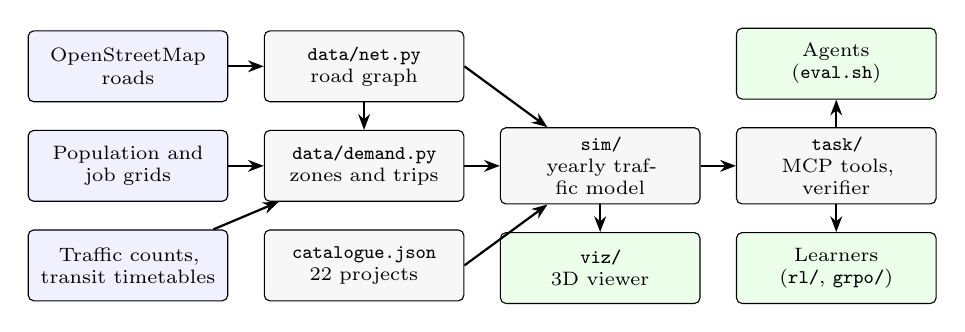
\begin{tikzpicture}[
  box/.style={draw, rounded corners=2pt, align=center, font=\scriptsize, minimum height=0.9cm, text width=2.3cm, fill=black!3},
  src/.style={box, fill=blue!6},
  res/.style={box, fill=green!8},
  arr/.style={-{Stealth[length=2mm]}, thick},
  node distance=0.35cm and 0.45cm]
\node[src] (osm) {OpenStreetMap\\roads};
\node[src, below=of osm] (hsy) {Population and\\job grids};
\node[src, below=of hsy] (tms) {Traffic counts,\\transit timetables};
\node[box, right=of osm] (net) {\texttt{data/net.py}\\road graph};
\node[box, right=of hsy] (dem) {\texttt{data/demand.py}\\zones and trips};
\node[box, right=of tms] (cat) {\texttt{catalogue.json}\\22 projects};
\node[box, right=of dem] (sim) {\texttt{sim/}\\yearly traffic model};
\node[box, right=of sim] (task) {\texttt{task/}\\MCP tools, verifier};
\node[res, above=of task] (agent) {Agents\\(\texttt{eval.sh})};
\node[res, below=of task] (learn) {Learners\\(\texttt{rl/}, \texttt{grpo/})};
\node[res, below=of sim] (viz) {\texttt{viz/}\\3D viewer};
\draw[arr] (osm) -- (net);
\draw[arr] (hsy) -- (dem);
\draw[arr] (tms) -- (dem);
\draw[arr] (net) -- (dem);
\draw[arr] (net.east) -- (sim);
\draw[arr] (dem) -- (sim);
\draw[arr] (cat.east) -- (sim);
\draw[arr] (sim) -- (task);
\draw[arr] (task) -- (agent);
\draw[arr] (task) -- (learn);
\draw[arr] (sim) -- (viz);
\end{tikzpicture}
\caption{The recipe as code, in the \repo{} repository. Public data (blue) becomes a road graph, a trip matrix and a list of projects. The simulator runs one year at a time. The task folder puts it behind four MCP tools and a verifier. Agents, learners and the 3D viewer (green) all use the same simulator. For a new city, the blue boxes change.}
\label{fig:repo}
\end{figure}

\repo{} is the recipe applied to Espoo and Kauniainen. It is an open repository, and every step of the recipe is a short Python script. Table~\ref{tab:repo} lists the folders. Below we give the Espoo choices for each step.

\begin{table}[t]
\caption{The folders of the repository.}
\label{tab:repo}
\centering\small
\begin{tabular}{@{}lp{0.72\linewidth}@{}}
\toprule
Folder & What it does \\
\midrule
\texttt{data/} & Downloads public data and builds the road graph, zones, trips and projects \\
\texttt{sim/} & The simulator: growth, money, road wear and the traffic equilibrium \\
\texttt{task/} & The test: task text, MCP server with four tools, reference solution, verifier \\
\texttt{rl/} & A small policy network, trained with behaviour cloning and PPO \\
\texttt{grpo/} & GRPO training of Gemma 3 (270M) with LoRA \\
\texttt{viz/} & A 3D viewer that replays runs \\
\texttt{eval.sh} & One command: reference, three agent runs, do nothing, stop early \\
\bottomrule
\end{tabular}
\end{table}

\textbf{Graph.} We read OpenStreetMap~\cite{haklay2008} for Espoo and Kauniainen, plus a 2.5\,km border. We keep the main road types (motorway to tertiary) and their ramps. When a road has no tag for lanes or speed, we use a default for its type. We keep only the largest part of the graph where every node can reach every other node. Roads that leave the area become \emph{gates}. The result has 10{,}706 one-way links.

\textbf{Zones.} We take the population grid~\cite{hsy2026a} and the job grid~\cite{hsy2026b} of the Helsinki region. Postal code data~\cite{statfi2026} gives the share of jobs that move goods. We split grid cells into zones of similar activity. Each zone links to the nearest road node. With the gates there are 117 zones.

\textbf{Trips.} We build a morning peak-hour trip matrix with a gravity model: more trips go between big zones that are close~\cite{ortuzar2011}. Public transport timetables~\cite{hsl2026} give transit times, and a logit model splits trips between car and transit. Traffic counts from 75 stations~\cite{fintraffic2026} give the flow at the gates and fix the free parameters. Then we adjust the matrix to the counts~\cite{vanzuylen1980}. Trucks get their own matrix from goods jobs.

\textbf{Check.} 75\% of the 75 stations have a GEH value below 10, and the model gives 1.02 times the counted flow. The code reports these numbers but sets no threshold. The usual target in practice is GEH below 5, so this fit is only moderate.

\textbf{Projects.} Twelve projects are real road plans of Espoo and the state, with cost and build time from public documents. Ten more are \emph{access upgrades}, one for each development area. These ten are defined by hand and all cost the same (Table~\ref{tab:cats}).

\textbf{Environment.} The simulator (\texttt{sim/}) runs one year per step. The MCP server (\texttt{task/}) gives the agent four tools and saves every year it commits. The task runs in Harbor~\cite{harbor2026}, and the agent connects with the Model Context Protocol~\cite{anthropic2024}. A verifier in a separate container replays the saved plan and computes the reward. One command, \texttt{SEED=0 ./eval.sh}, runs the full test: the reference, three agent runs, do nothing and an early stop. It needs Docker and Harbor 0.25; the README gives the steps. A web viewer replays the runs at \url{https://espoo.evinu.de}.

\begin{table}[t]
\caption{The 22 projects by type. Costs in MEUR.}
\label{tab:cats}
\centering\small
\begin{tabular}{@{}lrrr@{}}
\toprule
Type & Count & Cost & Build years \\
\midrule
\csname @@input\endcsname figs/cats.tex
\bottomrule
\end{tabular}
\end{table}

\section{The decision problem}\label{sec:model}

\begin{figure}[t]
  \centering
  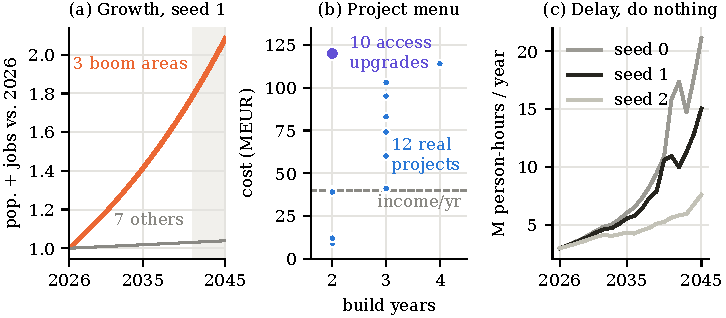
\includegraphics[width=\linewidth]{figs/problem.pdf}
  \caption{The problem. (a) Two or three of ten areas grow fast; which ones is hidden, but it shows in the yearly data. (b) Projects cost 9 to 120 MEUR and take 2 to 4 years; income is 40 MEUR a year. (c) If nothing is built, the yearly delay grows \nothingRatioMin{} to \nothingRatioMax{} times by 2045.}
  \label{fig:problem}
\end{figure}

This section describes the POMDP $\mathcal{M}_c$ that step 6 of the recipe produces. The definitions hold for any city; the numbers are those of Espoo. We drop the index $c$ to keep the notation short.

\textbf{The city.} The road network is a directed graph $G=(N,E)$. Each link $l\in E$ has a length $L_l$, a free speed $v_l$, a capacity $C_l$ and a condition $c_l\in[0,1]$. Trips go between zones. Let $q^{t}_{od}$ be the number of car trips from zone $o$ to zone $d$ in year $t$, and let $x_l$ be the flow on link $l$. The travel time on a link is the BPR function~\cite{bpr1964}:
\begin{equation}
t_l(x_l)=t^0_l\left(1+0.2\left(\frac{x_l}{C_l}\right)^4\right),\qquad t^0_l=\frac{L_l/v_l}{1-0.3\,(1-c_l)}.
\end{equation}
Bad roads are slower: a road in condition 0 has 30\% less free speed. Each year, the flows are at user equilibrium~\cite{wardrop1952}: for every pair $(o,d)$, all used routes have the same time, and no unused route is faster:
\begin{equation}
f_p>0 \;\Rightarrow\; \tau_p=\min_{p'\in P_{od}}\tau_{p'},\qquad \tau_p=\sum_{l\in p}t_l(x_l),
\end{equation}
where $P_{od}$ is the set of routes from $o$ to $d$ and $f_p$ is the flow on route $p$.

\textbf{The loss.} The delay in year $t$ is the time lost by all people in cars and trucks, compared with empty roads in perfect condition:
\begin{equation}
D_t=750\sum_{l\in E}\left(1.15\,x^{\text{car}}_l+x^{\text{truck}}_l\right)\left(t_l-\frac{L_l}{v_l}\right)\Big/60 \quad\text{person-hours per year}.
\end{equation}
Here 1.15 is the number of people per car, and 750 turns one peak hour into one year.

\textbf{Hidden growth.} There are ten development areas. A hidden set $B$ of two or three areas grows fast, at a rate $g_a$ between 3.2\% and 5.4\% a year. All other zones grow at 0.2\%. The agent does not see $B$, but it sees the population and jobs of every area each year. So $B$ can be found from the data.

\textbf{Money.} The agent starts with cash $k_0$ and gets an income $I=40$\,MEUR each year. A project with cost $K$ and $n$ build years costs $K/n$ per year. A start is allowed only if the cash stays at or above zero in every year of its payments. Maintenance at level $m\in\{0,1,2\}$ costs 0, 4 or 10\,MEUR a year. Roads that fall below condition 0.1 without repair need an emergency rebuild that costs four times as much.

\textbf{The POMDP.} Together, this is a POMDP $\mathcal{M}=(\mathcal{S},\mathcal{A},\mathcal{O},T,R,H)$ (Table~\ref{tab:pomdp}). The horizon is $H=20$ years (2026 to 2045). The agent acts in the first 15 years. In the last 5 years (the \emph{runout}) it cannot act, but the years still count. So a plan must also work after the agent stops.

\textbf{The score.} Let $D=\sum_{t}D_t$ be the total delay of a run, $D^{\varnothing}$ the total delay if the agent does nothing, and $D^{*}$ the lowest total delay we know for the same city. The score is
\begin{equation}
\text{score}=\operatorname{clip}_{[0,1]}\frac{D^{\varnothing}-D}{D^{\varnothing}-D^{*}}.
\end{equation}
Doing nothing scores 0, and the best known plan scores 1. On seeds 0 to 15, the best known plan saves \bestPctMin{}\% to \bestPctMax{}\% of $D^{\varnothing}$.

\begin{table}[t]
\caption{The POMDP. The agent observes the world through four MCP tools.}
\label{tab:pomdp}
\centering\small
\begin{tabular}{@{}p{0.14\linewidth}p{0.82\linewidth}@{}}
\toprule
Horizon & 20 yearly steps (2026 to 2045); actions only in the first 15 \\
State & lanes, speed, capacity and condition of each link; status of each project; cash and future payments; population and jobs per zone; the hidden set $B$ and rates $g_a$ \\
Action & up to 2 projects from 22, and a maintenance level $m\in\{0,1,2\}$; at most 762 joint actions; actions that do not fit the budget are rejected at no cost \\
Observation & \texttt{get\_state}: year, cash, payments, last delay, road condition, population and jobs per area (now and in 2026), startable projects, most delayed roads; \texttt{list\_projects}: cost, build years, running cost, status, \texttt{jam} (share of last year's delay on the project's roads); \texttt{forecast}: 4 plans per year, 3 years ahead; \texttt{commit\_year} \\
Transition & growth of people and jobs; payments; road works cut capacity until the project opens; condition falls, maintenance repairs the worst roads; new traffic equilibrium \\
Reward & $r_t=(D^{\varnothing}_t-D_t)/(D^{\varnothing}-D^{*})$; the score is the clipped sum \\
\bottomrule
\end{tabular}
\end{table}

\textbf{Why the task is hard.} The hard part is not to see the growth. It is to act on it early. An access upgrade costs 120\,MEUR, three years of income. It closes roads for two years before it helps. A 3-year forecast shows mostly the road works, and the benefit comes later. A good agent must save money and build before the traffic gets bad.

\textbf{Why the reward is hard to game.} (1) Doing nothing scores 0; measured do-nothing scores stay below \nothingAbsMax{} on 16 seeds. (2) The agent never reports a score. The server saves each year, and the verifier replays the plan from the start in a separate container. (3) Stopping early does not help: the rest of the years run with no new projects and default maintenance. If the reference plays only the first 3 years and stops, it scores 0.05 on seed 0 (0.05 to 0.38 on seeds 0 to 4). (4) A rejected action does nothing and costs nothing, so testing the rules gives no gain. (5) Only 4 forecasts per year, 3 years ahead, so the agent cannot search all plans through the tools. (6) The task text states the same rules as the simulator. (7) On machines with the same CPU, a replay gives exactly the same delays. Across CPU types, rounding changes the total delay by at most 0.24\% and the score by at most 0.008, far below the gap between methods.

\section{Learning methods}\label{sec:learn}

This section gives the technical details of the two learners that we train in the environment: a small policy network (Section~\ref{sec:poc}) and a language model trained with GRPO (Section~\ref{sec:grpo}).

\subsection{The policy network}

\begin{figure}[t]
\centering
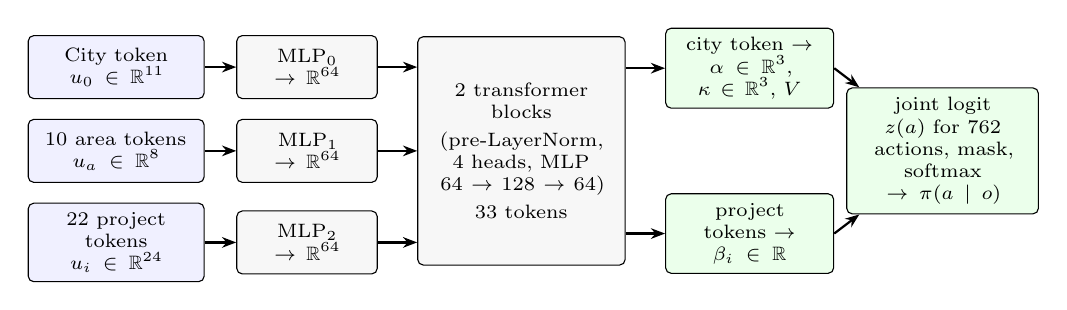
\begin{tikzpicture}[
  bx/.style={draw, rounded corners=2pt, align=center, font=\scriptsize, minimum height=0.8cm, fill=black!3},
  inp/.style={bx, fill=blue!6, text width=2.0cm},
  emb/.style={bx, text width=1.55cm},
  hd/.style={bx, fill=green!8, text width=1.9cm},
  arr/.style={-{Stealth[length=1.8mm]}, thick},
  node distance=0.25cm and 0.4cm]
\node[inp] (g) {City token\\$u_0\in\mathbb{R}^{11}$};
\node[inp, below=of g] (a) {10 area tokens\\$u_a\in\mathbb{R}^{8}$};
\node[inp, below=of a] (p) {22 project tokens\\$u_i\in\mathbb{R}^{24}$};
\node[emb, right=of g] (eg) {MLP$_0$\\$\to\mathbb{R}^{64}$};
\node[emb, right=of a] (ea) {MLP$_1$\\$\to\mathbb{R}^{64}$};
\node[emb, right=of p] (ep) {MLP$_2$\\$\to\mathbb{R}^{64}$};
\node[bx, right=0.5cm of ea, text width=2.4cm, minimum height=2.9cm] (tr) {2 transformer\\blocks\\[2pt](pre-LayerNorm,\\4 heads, MLP\\$64\to128\to64$)\\[2pt]33 tokens};
\node[hd, right=0.5cm of tr, yshift=1.05cm] (h1) {city token $\to$\\$\alpha\in\mathbb{R}^3$, $\kappa\in\mathbb{R}^3$, $V$};
\node[hd, right=0.5cm of tr, yshift=-1.05cm] (h2) {project tokens $\to$\\$\beta_i\in\mathbb{R}$};
\node[hd, right=0.45cm of tr, xshift=2.35cm, text width=2.2cm, minimum height=1.6cm] (j) {joint logit\\$z(a)$ for 762\\actions, mask,\\softmax $\to\pi(a\mid o)$};
\draw[arr] (g) -- (eg); \draw[arr] (a) -- (ea); \draw[arr] (p) -- (ep);
\draw[arr] (eg.east) -- (tr.west |- eg.east); \draw[arr] (ea) -- (tr); \draw[arr] (ep.east) -- (tr.west |- ep.east);
\draw[arr] (tr.east |- h1) -- (h1); \draw[arr] (tr.east |- h2) -- (h2);
\draw[arr] (h1.east) -- (j); \draw[arr] (h2.east) -- (j);
\end{tikzpicture}
\caption{The policy network (82{,}760 parameters). Each kind of token has its own small MLP. A transformer~\cite{vaswani2017} lets every token look at every other token. The city token gives the maintenance logits $\alpha$, the build-count logits $\kappa$ and the value $V$; each project token gives one logit $\beta_i$. Together they score each of the 762 joint actions (Equation~\ref{eq:joint}).}
\label{fig:policy}
\end{figure}

\textbf{Input.} The observation $o_t$ comes only from the tools \texttt{get\_state} and \texttt{list\_projects}. It becomes 33 tokens: one city token $u_0$ (time, cash, payments, running costs, car share, road condition, last delay), one token $u_a$ per area (size in 2026, growth so far, yearly growth rate, position) and one token $u_i$ per project (kind, cost, build time, running cost, status, position, growth near the project, \texttt{jam}).

\textbf{Network.} Each kind of token has its own two-layer MLP that maps it to $\mathbb{R}^{64}$. Then two transformer blocks~\cite{vaswani2017} with LayerNorm before each part update all tokens:
\begin{equation}
X\leftarrow X+\operatorname{MHA}(\operatorname{LN}(X)),\qquad X\leftarrow X+\operatorname{MLP}(\operatorname{LN}(X)),
\end{equation}
with multi-head attention (4 heads, $d_k=16$)
\begin{equation}
\operatorname{Attention}(Q,K,V)=\operatorname{softmax}\!\left(\frac{QK^\top}{\sqrt{d_k}}\right)V .
\end{equation}
There is no position encoding: the tokens carry their map position as features, and the order of areas and projects does not matter. Figure~\ref{fig:policy} shows the network.

\textbf{Joint actions.} An action $a=(m,i,j)$ is a maintenance level $m\in\{0,1,2\}$ and up to two projects $i<j$, where $\varnothing$ means ``no project''. With 22 projects there are $3\,(1+22+\binom{22}{2})=762$ actions. The network scores each action as a sum of parts:
\begin{equation}\label{eq:joint}
z(a)=\alpha_m+\kappa_{n(a)}+\beta_i+\beta_j,\qquad \beta_\varnothing=0,\qquad
\pi_\theta(a\mid o)=\frac{\mathbf{1}[a\in\mathcal{F}(o)]\,e^{z(a)}}{\sum_{a'\in\mathcal{F}(o)}e^{z(a')}},
\end{equation}
where $n(a)\in\{0,1,2\}$ is the number of projects in $a$ and $\mathcal{F}(o)$ is the set of actions that fit the budget. At test time the policy takes $\arg\max_a z(a)$.

\textbf{Behaviour cloning.} We first copy expert plans found by search on training seeds. For expert actions $a^*$ and returns $G_t$ we minimise
\begin{equation}
\mathcal{L}_{\text{BC}}(\theta)=\mathbb{E}\left[-\log\pi_\theta(a^*_t\mid o_t)+\left(V_\theta(o_t)-G_t\right)^2\right].
\end{equation}

\textbf{PPO.} We then fine-tune with PPO~\cite{schulman2017}. The reward of year $t$ is the saved delay, $r_t=(D^{\varnothing}_t-D_t)/\bar D^{\varnothing}$, where $\bar D^{\varnothing}$ is the mean yearly do-nothing delay. Advantages use GAE~\cite{schulman2016} with $\gamma=1$ and $\lambda=0.95$:
\begin{equation}
\delta_t=r_t+V(o_{t+1})-V(o_t),\qquad \hat A_t=\sum_{k\ge 0}\lambda^k\,\delta_{t+k}.
\end{equation}
With the ratio $\rho_t(\theta)=\pi_\theta(a_t\mid o_t)/\pi_{\theta_{\text{old}}}(a_t\mid o_t)$ and $\epsilon=0.2$, the loss is
\begin{equation}
\begin{aligned}
\mathcal{L}_{\text{PPO}}(\theta)={}&-\mathbb{E}_t\!\left[\min\!\left(\rho_t\hat A_t,\;\operatorname{clip}(\rho_t,1-\epsilon,1+\epsilon)\,\hat A_t\right)\right]\\
&+0.5\,\mathbb{E}_t\!\left[\left(V_\theta(o_t)-\hat G_t\right)^2\right]-0.01\,\mathbb{E}_t\,\mathcal{H}\!\left[\pi_\theta(\cdot\mid o_t)\right],
\end{aligned}
\end{equation}
where $\hat G_t=\hat A_t+V(o_t)$ and $\mathcal{H}$ is the entropy. We normalise $\hat A_t$ over the batch and use 4 epochs per update.

\subsection{GRPO for the language model}

GRPO~\cite{shao2024} is PPO without a value network. Instead of $V(o)$, it compares several answers to the same prompt. For a prompt $q$, it samples a group of $G$ answers $o_1,\dots,o_G$ from the old policy, scores each answer with a reward $r_i$, and normalises the rewards inside the group:
\begin{equation}\label{eq:grpoadv}
\hat A_{i,t}=\frac{r_i-\operatorname{mean}(r_1,\dots,r_G)}{\operatorname{std}(r_1,\dots,r_G)}.
\end{equation}
Every token $t$ of answer $i$ gets the same advantage. The GRPO objective is
\begin{equation}\label{eq:grpo}
\begin{aligned}
\mathcal{J}_{\text{GRPO}}(\theta)=\mathbb{E}_{q,\{o_i\}}\Bigg[\frac{1}{G}\sum_{i=1}^{G}\frac{1}{|o_i|}\sum_{t=1}^{|o_i|}\Big(&\min\!\big(\rho_{i,t}\hat A_{i,t},\;\operatorname{clip}(\rho_{i,t},1-\epsilon,1+\epsilon)\,\hat A_{i,t}\big)\\
&-\beta\,\mathbb{D}_{\text{KL}}\!\left[\pi_\theta\,\|\,\pi_{\text{ref}}\right]\Big)\Bigg],
\end{aligned}
\end{equation}
with the token ratio
\begin{equation}
\rho_{i,t}=\frac{\pi_\theta(o_{i,t}\mid q,o_{i,<t})}{\pi_{\theta_{\text{old}}}(o_{i,t}\mid q,o_{i,<t})},
\end{equation}
and the KL term estimated per token as $\frac{\pi_{\text{ref}}}{\pi_\theta}-\log\frac{\pi_{\text{ref}}}{\pi_\theta}-1$~\cite{shao2024}. DeepSeek-R1 uses the same objective with rule-based rewards~\cite{guo2025}.

\textbf{Our case.} We use $\beta=0$ (no KL term) and one gradient step per batch, so $\pi_{\theta_{\text{old}}}=\pi_\theta$ when we take the gradient. Then $\rho_{i,t}=1$, the clip is never active, and the gradient of Equation~\ref{eq:grpo} becomes a policy gradient with the group advantage:
\begin{equation}\label{eq:ourgrpo}
\nabla_\theta\mathcal{J}(\theta)=\frac{1}{N}\sum_{q}\sum_{i=1}^{G}\sum_{t=1}^{|o_i|}\hat A_{i}\,\nabla_\theta\log\pi_\theta(o_{i,t}\mid q,o_{i,<t}),
\end{equation}
where $N$ is the number of answer tokens in the batch (we average over all tokens, not per answer). The reward of an answer is
\begin{equation}
r_i=\operatorname{clip}_{[-0.5,\,1.5]}\!\left(\frac{1}{0.3}\cdot\frac{D^{\varnothing}-D(o_i)}{D^{\varnothing}}-0.05\,b_i\right),
\end{equation}
where $D(o_i)$ is the total delay when the environment plays the plan in $o_i$, and $b_i$ counts wrong project names (and a missing maintenance level). An answer that cannot be read gets $-0.5$. We use $G=8$ answers for each of 4 prompts per step, sampling temperature 1, and learning rate $2\cdot10^{-5}$.

\textbf{LoRA.} We do not change the weights $W_0$ of Gemma. We train a low-rank update in every linear layer~\cite{hu2022}:
\begin{equation}
W=W_0+\frac{\alpha}{r}\,BA,\qquad B\in\mathbb{R}^{d\times r},\;A\in\mathbb{R}^{r\times k},\;r=16,\;\alpha=32 .
\end{equation}

\textbf{A note on Equation~\ref{eq:grpoadv}.} If all $G$ answers in a group get the same reward, every $\hat A_i$ is zero, and by Equation~\ref{eq:ourgrpo} the group gives no gradient. We will see that this is exactly what stops our training (Section~\ref{sec:grpo}).

\section{Proof of concept: a frontier agent fails}\label{sec:poc}

\begin{figure}[t]
  \centering
  \begin{subfigure}{0.49\linewidth}\shot{heat0}\caption{Delay, 2026}\end{subfigure}\hfill
  \begin{subfigure}{0.49\linewidth}\shot{heat19}\caption{Delay, 2045, do nothing}\end{subfigure}
  \caption{The 3D viewer replays runs (seed 1). Colour shows delay per road, from green (free) to purple (jammed). Without action, jams spread from the growing areas by 2045.}
  \label{fig:viewer}
\end{figure}

\textbf{Methods.} We compare seven ways to play:
\begin{itemize}
\item \emph{Do nothing} and \emph{Random} (a random allowed action each year).
\item \emph{Greedy}: forecast each project alone and start the best two per euro, judged 1 year or 5 years after opening.
\item \emph{Reactive}: build where the delay was highest last year.
\item \emph{Rule planner}: a short hand-written rule with no forecasts. It upgrades the access of each area that grows clearly faster than the base rate.
\item \emph{Frontier agent}: \texttt{gpt-6.1-sol} in the OpenCode harness~\cite{opencode2025}, with the task text and the four tools. A run takes \agentMinMin{} to \agentMinMax{} minutes and costs \$\agentUsdMin{} to \$\agentUsdMax{}.
\item \emph{Learned policy}: a small transformer~\cite{vaswani2017} with 82{,}760 parameters. It reads one token for the city, one per area and one per project, all from the tools (Figure~\ref{fig:policy}). We train it with behaviour cloning on plans found by search (seeds 1000 and up), then with PPO~\cite{schulman2017} (seeds 2000 and up); see Section~\ref{sec:learn}. It uses no forecasts. Two variants add tools to it: \emph{forecast check} tests its top 4 actions with the 4 allowed forecasts, and \emph{search} adds Gumbel search~\cite{danihelka2022} outside the tool limits.
\end{itemize}
We test on seeds 0 to 15, and we check the learned policy on \hoN{} more scenarios that we never used for training or for choosing a checkpoint.

\begin{table}[t]
\caption{Results. Scores are means over seeds 0 to 15 and over the agent's seeds (\agentSeeds{}). The other columns use the agent's seeds: total person-hours lost and saved over 20 years, delay in the final year, and money spent. --: not logged.}
\label{tab:main}
\centering\small
\begin{tabular}{@{}lrrrrrrr@{}}
\toprule
 & \multicolumn{2}{c}{Score} & Lost & \multicolumn{2}{c}{Saved} & 2045 delay & Spend \\
\cmidrule(lr){2-3}\cmidrule(lr){5-6}
Method & 16 seeds & agent's & M p-h & M p-h & \% & M p-h/yr & MEUR \\
\midrule
\csname @@input\endcsname figs/table.tex
\bottomrule
\end{tabular}
\end{table}

\begin{figure}[t]
  \centering
  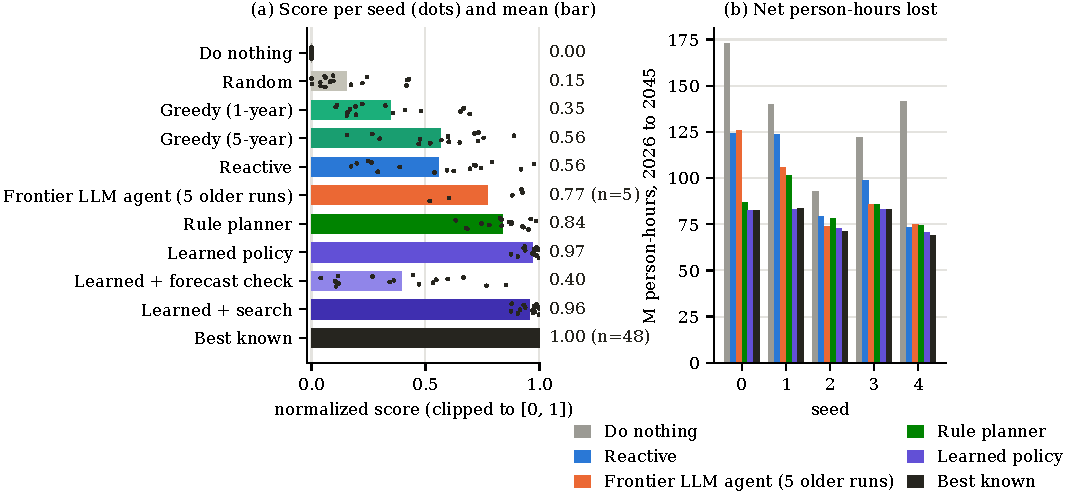
\includegraphics[width=\linewidth]{figs/bars.pdf}
  \caption{(a) Score per seed (dots) and mean (bar). (b) Person-hours lost from 2026 to 2045; lower is better.}
  \label{fig:bars}
\end{figure}

\textbf{Main result.} Table~\ref{tab:main} and Figure~\ref{fig:bars} show the results. Doing nothing is the worst plan. Random plans help a little. Greedy plans help in some scenarios and fail in others, because they judge each project alone and over a short time. The frontier agent scores \agentScoreMean{}. The simple rule planner scores 0.84, and the learned policy scores \rlScore{}, both without forecasts. Through Harbor, the learned policy gives the same delays as our own simulator. On \hoN{} unseen scenarios the learned policy saves \hoRl{}\% of the do-nothing delay (\hoRlEval{}\% on seeds 0 to 15), and it beats the rule planner in \hoWinPlanner{} of \hoN{} scenarios (Table~\ref{tab:heldout}).

\begin{table}[t]
\caption{Share of the do-nothing delay saved (\%), on \hoN{} unseen scenarios and on seeds 0 to 15.}
\label{tab:heldout}
\centering\small
\begin{tabular}{@{}lrrr@{}}
\toprule
 & \multicolumn{2}{c}{Unseen scenarios} & Seeds 0 to 15 \\
\cmidrule(lr){2-3}
Method & mean & worst & mean \\
\midrule
\csname @@input\endcsname figs/heldout.tex
\bottomrule
\end{tabular}
\end{table}

\begin{figure}[t]
  \centering
  \begin{minipage}[b]{0.49\linewidth}\centering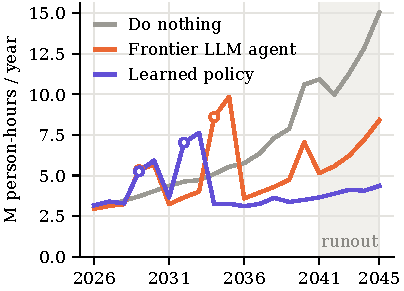
\includegraphics[width=\linewidth]{figs/years.pdf}\end{minipage}\hfill
  \begin{minipage}[b]{0.49\linewidth}\centering\shot{split}\end{minipage}
  \caption{Seed 1. Left: yearly delay; circles mark the start of access upgrades. Right: the delay map in 2045, learned policy (left of the line) against the frontier agent (right).}
  \label{fig:fail}
\end{figure}

\textbf{How the frontier agent fails.} The agent's plan hardly depends on the scenario:
\begin{enumerate}
\item \textbf{One list for every scenario.} Every run starts the two cheap links \texttt{olari-link} and \texttt{mankkaa-link}, then \texttt{espoonvayla-2x2} and \texttt{otaniemi-access}. Otaniemi grows fast in only two of these scenarios.
\item \textbf{Late answer to growth.} Of the \nBooms{} fast-growing areas, it upgrades \agentBoomHits{}, and only \agentBoomEarly{} by 2031. A second access upgrade comes in 2034 or never.
\item \textbf{It trusts short forecasts and reads little data.} It calls \texttt{get\_state} only \agentGetStateMin{} to \agentGetStateMax{} times in 20 years, but it makes \agentForecastMin{} to \agentForecastMax{} forecasts.
\end{enumerate}
The learned policy starts two access upgrades in every scenario and reaches a growing area by 2029 in \rlBoomEarly{} of \rlN{} scenarios (Figure~\ref{fig:fail}). In seed 0 the agent loses \gapRlA{}M person-hours more than the learned policy. Per seed, the agent scores 0.52, 0.60, 0.88, 0.93 and 0.92 on seeds 0 to 4, against 1.00, 1.00, 0.91, 0.99 and 0.98 for the learned policy. So the agent loses a lot where growth needs an early answer (seeds 0 and 1), and only 0.03 to 0.06 where its generic plan happens to fit (seeds 2 to 4).

\textbf{The forecast is a trap.} A 3-year forecast of a 120\,MEUR upgrade shows two years of road works and little gain. If the learned policy checks its top 4 choices with the same forecasts and keeps the best, its score falls from \rlScore{} to \rlcheckScore{}. The forecast is not wrong. Its window is too short for the decision. This is the trap the frontier agent falls into. The agent has all the information it needs: the growth is in \texttt{get\_state}, and the rules are in the task text. It fails because of its decisions.

\section{GRPO: the model learns from the reward, then takes a shortcut}\label{sec:grpo}

Can a small language model learn this task from the environment alone? We train \texttt{gemma-3-270m-it}~\cite{gemmateam2025} with LoRA~\cite{hu2022} (rank 16) and GRPO~\cite{shao2024,guo2025} on a CPU.

\textbf{Setup.} We make the task single-turn, so that one answer is one full plan. The environment first runs two years, so that growth shows. The prompt gives the budget, the growth of each area so far (fastest first) and the projects with cost, build time and nearest area. The model writes one line: \texttt{plan: id, id, ...; maintain: k}. The environment starts the projects in this order when the budget allows, at most two per year. The reward, the GRPO update and LoRA are in Section~\ref{sec:learn} (Equations~\ref{eq:grpoadv}--\ref{eq:ourgrpo}). A short warm-up (120 steps) on random valid plans teaches only the answer format. We train on seeds 1000 to 1399 and test on seeds 0 to 15.

\begin{figure}[t]
  \centering
  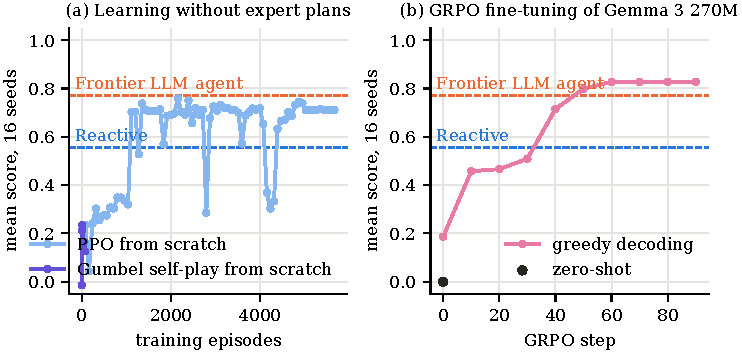
\includegraphics[width=\linewidth]{figs/curves.pdf}
  \caption{Training curves, mean score on 16 seeds. (a) The policy network trained from scratch, without expert plans. (b) GRPO on Gemma 3 270M. Dashed: frontier agent and reactive rule.}
  \label{fig:curves}
\end{figure}

\textbf{It learns.} Without training, Gemma never writes a valid answer (score \grpoZero{}). After the warm-up it scores \grpoWarm{}. After \grpoSteps{} GRPO steps it scores \grpoFinal{}, with \grpoValid{} of the answers valid (Figure~\ref{fig:curves}b). This is close to the rule planner. It is also above the frontier agent, but the comparison is not fair: Gemma plays an easier single-turn version, and the first two years are played for it. It learns in a clear order: first the format, then the best maintenance level ($m=2$, from step \grpoMtwoAt{}), then a fixed set of good projects (from step \grpoKeptAt{}).

\textbf{Then it takes a shortcut.} After training, Gemma writes the \emph{same} plan for all 16 test scenarios: \grpoPlan{}. It does not read the growth in the prompt. Only \grpoBoomShare{} of its access upgrades are in growing areas. The plan scores well because Otaniemi and Kiviruukki are often among the growing areas, so it works on average. This is a shortcut~\cite{geirhos2020}: the model fits the average scenario, not the one in front of it.

\textbf{Two separate facts.} It is important to keep two things apart. First, \emph{the model learns from the reward}: the score goes from \grpoZero{} to \grpoFinal{}, and each step of learning (format, maintenance, good projects) follows the reward. So the environment gives a useful training signal. Second, \emph{the reward is satisfied by a plan that ignores the input}. This is overfitting: the model fits the training scenarios with one answer instead of a rule that reads the city.

\textbf{The shortcut belongs to one city.} The learned answer is a list of names: \texttt{otaniemi-access}, \texttt{kiviruukki-access}, \texttt{espoonvayla-2x2}. These names exist only in Espoo's project list $K_c$. All 400 training scenarios share this list, the same graph and the same ten areas, so a fixed list of names can be right on average. In a training set with many cities, each city has its own projects and areas. A fixed list of names would then be wrong in most cities, and the only way to score well would be to read the prompt. In this sense, a multi-city version removes this shortcut by construction.

\textbf{Not the only cause.} One city is not the whole story. The policy network is trained only on Espoo too, but it reads the growth and works on \hoN{} unseen scenarios (Section~\ref{sec:poc}). So the signal can be learned from one city. The GRPO setup also matters: the task is single-turn, and the groups lose their variety, as we show next.

\textbf{Why learning stops.} At step \grpoOneAt{}, the 8 answers for a scenario become almost the same plan. From step \grpoFlatAt{}, all answers in a group get the same reward. Then every advantage $\hat A_i$ in Equation~\ref{eq:grpoadv} is zero, and by Equation~\ref{eq:ourgrpo} the gradient is zero. The model cannot find a better plan, because it no longer tries other plans. The score stays at \grpoScoreEnd{} until the end.

\begin{figure}[t]
  \centering
  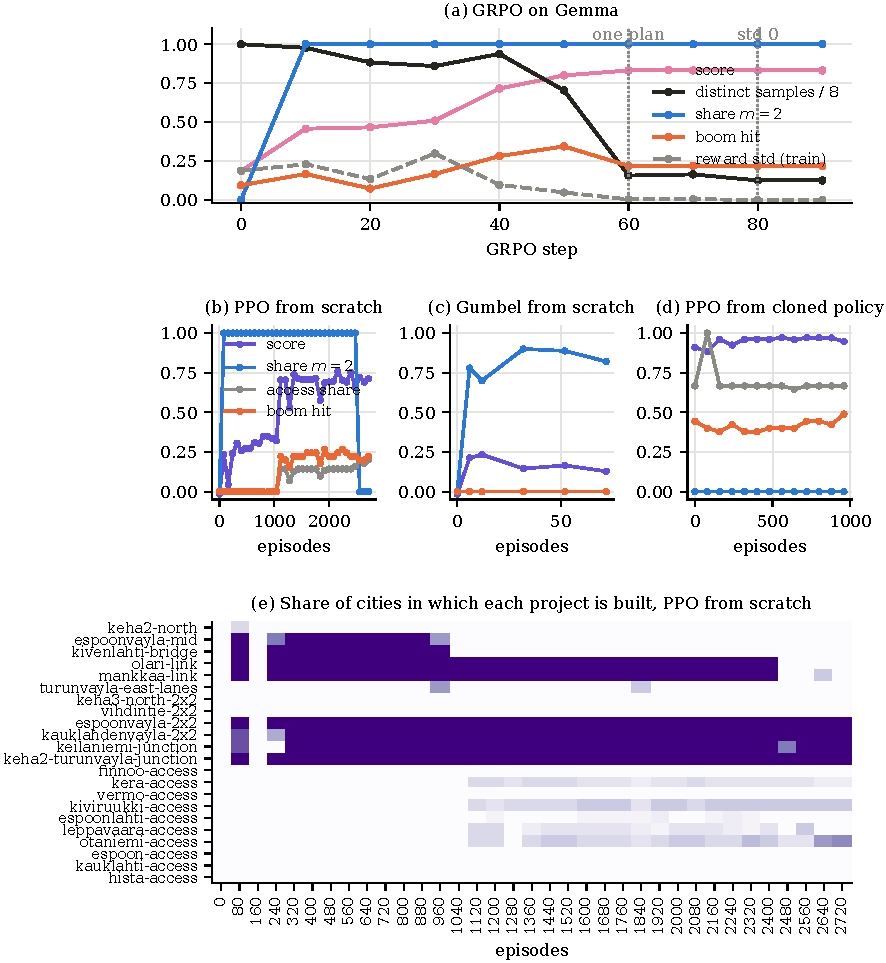
\includegraphics[width=\linewidth]{figs/evolution.pdf}
  \caption{How the strategy changes during training, on the plans for seeds 0 to 15 at each checkpoint. (a) GRPO on Gemma 3 270M. (b to d) The policy network trained with RL from scratch (PPO, Gumbel self-play) and from the cloned policy (PPO). (e) Which projects the RL policy builds at each checkpoint.}
  \label{fig:evolution}
\end{figure}

\textbf{The same order for every learner.} The policy network shows the same pattern (Figure~\ref{fig:evolution}). Trained from scratch with PPO, it first finds the maintenance level and cheap roads, and adds access upgrades only after \evoColdNoAccUntil{} episodes, and then too late (score \evoColdScore{} after \evoColdEps{} episodes). Only the policy that starts from expert plans upgrades the growing areas early. The frontier agent also stops at the generic stage. All learners find the easy parts first: a valid answer, the maintenance level and a generic list of good projects. The hard part is to read the growth and build early.

\section{Discussion: many cities from one recipe}\label{sec:scale}

This paper is a proof of concept. We defined the recipe, built one instance, showed a clear failure of a frontier agent, and showed that a small language model learns from the reward. The next question is how to make GRPO learn the hard part: read the growth and build early. We think the main answer is more varied training data, and the recipe is a way to produce it. This is a hypothesis; we have not tested it yet.

\textbf{Evidence from RL.} In deep RL, agents trained on few levels memorise them, and the gap between training and test falls as the number of different training levels grows~\cite{zhang2018,cobbe2019,cobbe2020,kirk2023}. Domain randomisation uses the same idea with random versions of a simulator~\cite{tobin2017}. In our setting, each city is like a level, and each seed is a variation inside it. The difference is that our levels are real cities.

\textbf{One city is not varied enough.} With ten areas and two or three of them growing fast, there are only $\binom{10}{2}+\binom{10}{3}=165$ possible sets of growing areas. The graph, the projects and the costs are the same in every scenario. So one list of project names that fits the most common areas can score well everywhere.

\textbf{What the recipe can add.}
\begin{enumerate}
\item \textbf{More cities.} Each city run through the recipe brings a new graph, new zones, new areas and new projects. Roads and timetables exist in the same format for many cities (Table~\ref{tab:inputs}); counts, jobs and project lists need more work per country.
\item \textbf{More variation inside a city.} Seeds can also change project costs, build times, the budget, the number of growing areas and the base growth. Then no single plan is good everywhere, even in one city.
\item \textbf{Keep the groups diverse.} GRPO stops when all answers in a group get the same reward. Larger groups, a higher sampling temperature, or dropping prompts with equal rewards~\cite{yu2025} keep the gradient alive.
\item \textbf{Multi-turn play.} In the full task the agent sees the city every year. A multi-turn version would let the model react to growth instead of guessing it in year two.
\end{enumerate}
If the hypothesis holds, a small open model trained on many cities would have to read the growth, as the policy network does, and could beat the frontier agent with far less compute. The test is clear: train GRPO on scenarios from several cities and evaluate it on a city it has never seen.

\section{Limitations}

\textbf{The recipe.} We applied it to one city only, so its generality is a claim, not a result. Some of its inputs (jobs, counts, real projects) depend on the country, and the list of real projects is made by hand. We have not fixed the thresholds $\alpha$ and $\beta$ yet.

\textbf{The model.} The traffic model is a static equilibrium for one peak hour, scaled to a year. It has no queues and no time of day. The car share is fixed, so better roads do not pull people out of transit. The ten access upgrades are generated and have the same cost. $D^{*}$ is the best plan we know, not a proven best plan.

\textbf{The experiments.} The frontier agent ran once on each of \agentN{} seeds, so its mean is uncertain. Its runs were made before we froze $D^{*}$ in \texttt{sim/norms.json}; we rescored their delays with the frozen values. We chose the policy checkpoint on the test seeds; on unseen scenarios it saves \hoGap{} points less. GRPO used one small model, one setting and a CPU.

\section{Conclusion}

We proposed a recipe that turns the public data of a city into a planning test for AI agents, with a formal definition, a check against real traffic counts, and a reward that a separate program replays. Its first instance, \repo{}, is an open repository for Espoo with one command to run everything. In this proof of concept, a frontier agent uses one generic plan and answers growth too late, while a small trained policy avoids this trap. A 270M language model trained with GRPO learns from the reward, but it finds a shortcut: one list of Espoo project names for every scenario. A training set with many cities, built by the same recipe, removes this shortcut by construction. We believe this is the way to train small models that really read the city before they build.

\bibliographystyle{plainnat}
\bibliography{refs}

\end{document}
